
% MATH -------------------------------------------------------------------
\newcommand{\A}{{\cal A}}
\newcommand{\h}{{\cal H}}
\newcommand{\s}{{\cal S}}
\newcommand{\W}{{\cal W}}
\newcommand{\BH}{\mathbf B(\cal H)}
\newcommand{\KH}{\cal  K(\cal H)}
\newcommand{\Real}{\mathbb R}
\newcommand{\Complex}{\mathbb C}
\newcommand{\Field}{\mathbb F}
\newcommand{\RPlus}{[0,\infty)}
%
\newcommand{\norm}[1]{\left\Vert#1\right\Vert}
\newcommand{\essnorm}[1]{\norm{#1}_{\text{\rm\normalshape ess}}}
\newcommand{\abs}[1]{\left\vert#1\right\vert}
\newcommand{\set}[1]{\left\{#1\right\}}
\newcommand{\seq}[1]{\left<#1\right>}
\newcommand{\eps}{\varepsilon}
\newcommand{\To}{\longrightarrow}
\newcommand{\RE}{\operatorname{Re}}
\newcommand{\IM}{\operatorname{Im}}
\newcommand{\Poly}{{\cal{P}}(E)}
\newcommand{\EssD}{{\cal{D}}}
% THEOREMS ---------------------------------------------------------------
\theoremstyle{plain}
\newtheorem{thm}{Theorem}[section]
\newtheorem{cor}[thm]{Corollary}
\newtheorem{lem}[thm]{Lemma}
\newtheorem{prop}[thm]{Proposition}

\theoremstyle{definition}
\newtheorem{defn}{Definition}[section]
%
\theoremstyle{remark}
\newtheorem{rem}{Remark}[section]
%
\def\baselinestretch{1}

\chapter{Appendix }

\def\baselinestretch{1.66}

\begin{figure}[H]
\centering
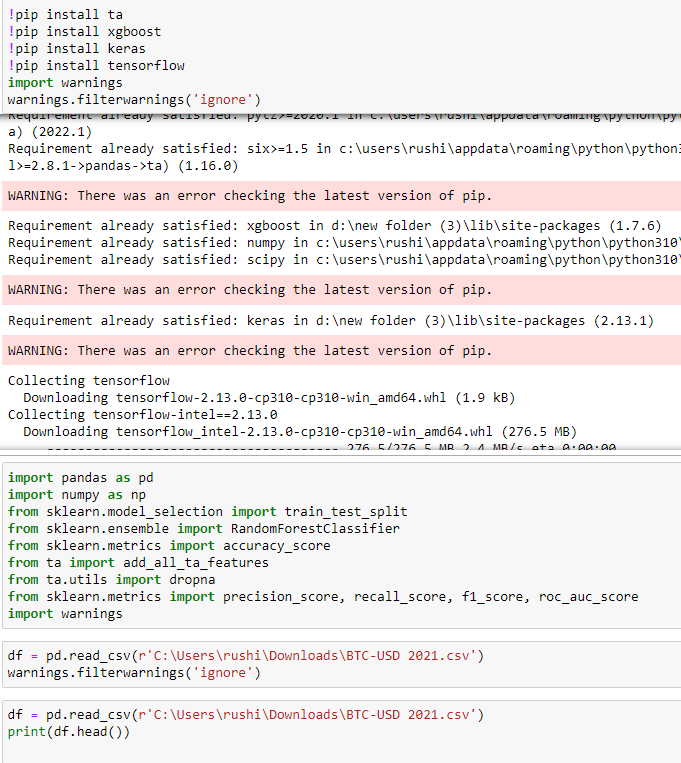
\includegraphics[scale=0.75]{fig16.jpg}

\end{figure}

\begin{figure}[H]
\centering
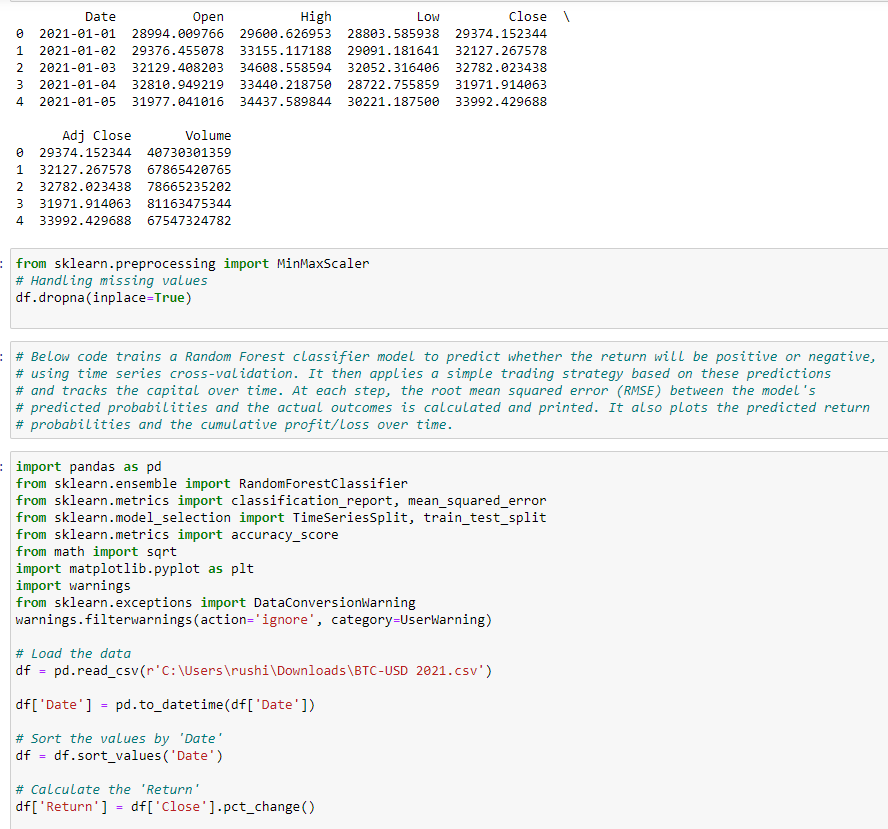
\includegraphics[scale=0.65]{fig17.jpg}
\end{figure}

\begin{figure}[H]
\centering
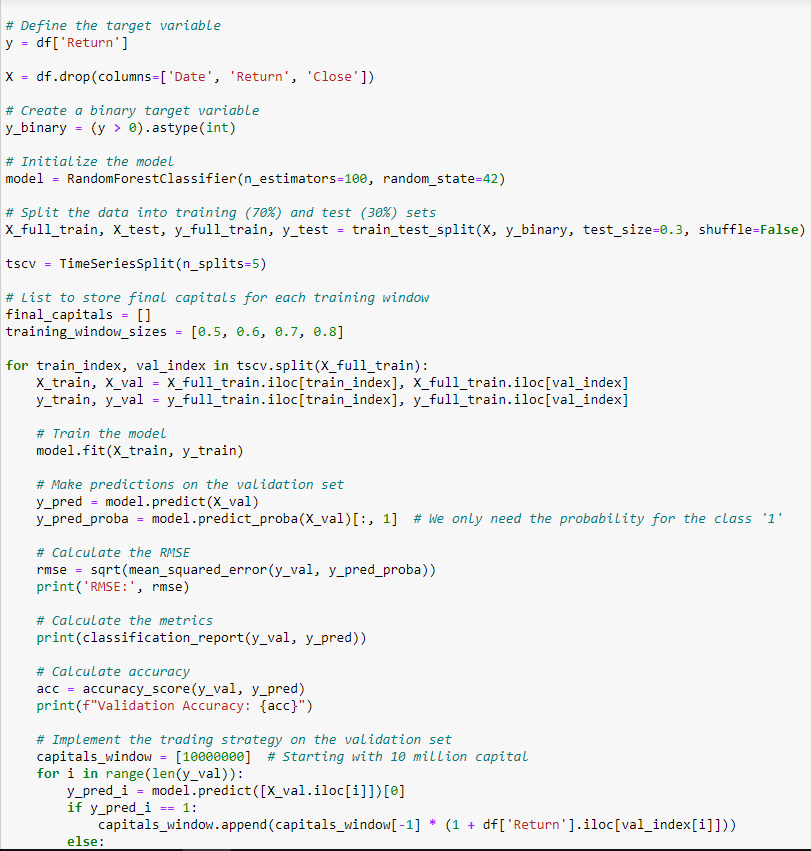
\includegraphics[scale=0.75]{fig18.jpg}

\end{figure}

\begin{figure}[H]
\centering
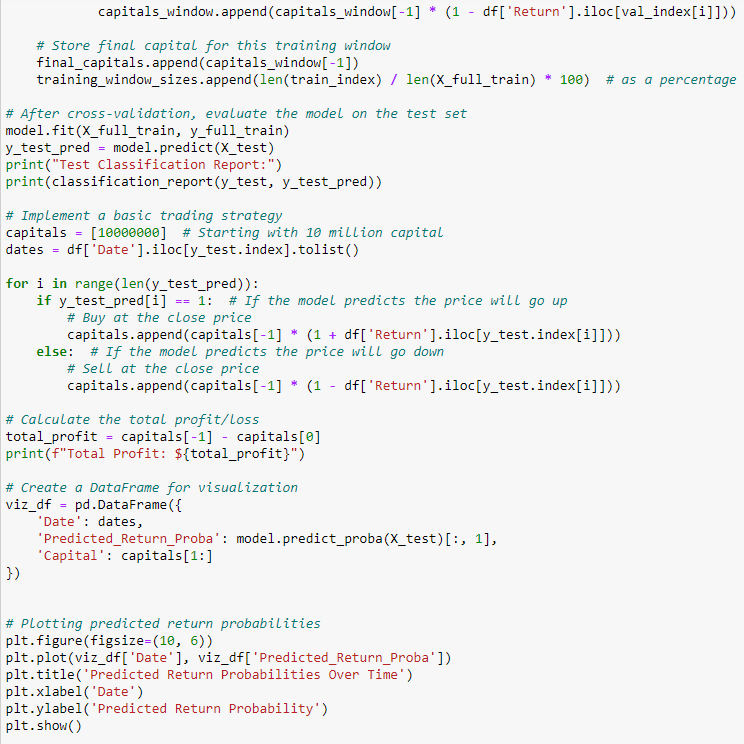
\includegraphics[scale=0.75]{fig19.jpg}

\end{figure}

\begin{figure}[H]
\centering
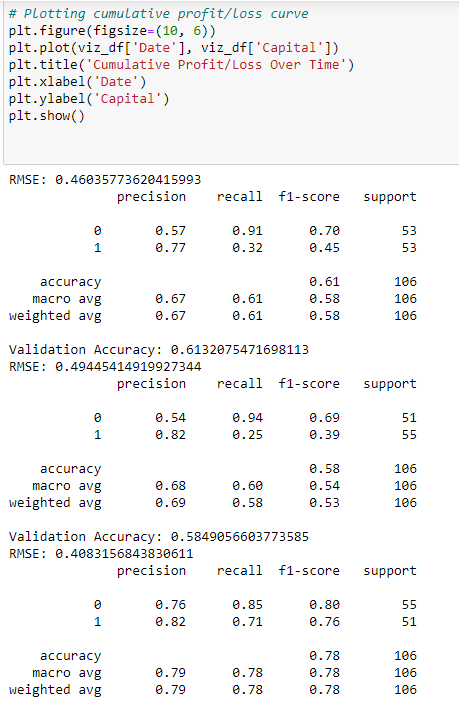
\includegraphics[scale=0.65]{fig20.jpg}
\end{figure}

\begin{figure}[H]
\centering
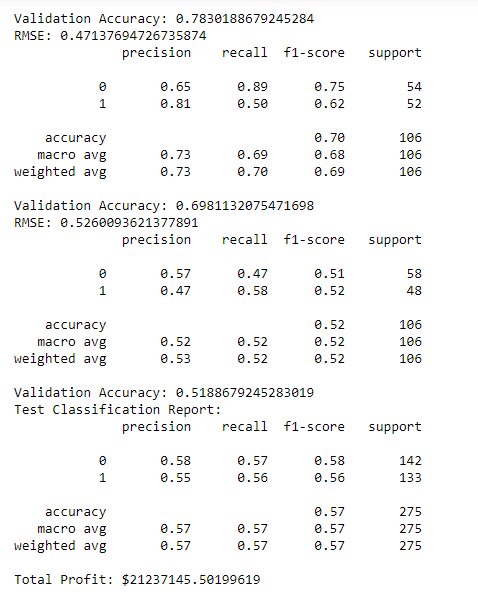
\includegraphics[scale=0.65]{fig21.jpg}
\end{figure}

\begin{figure}[H]
\centering
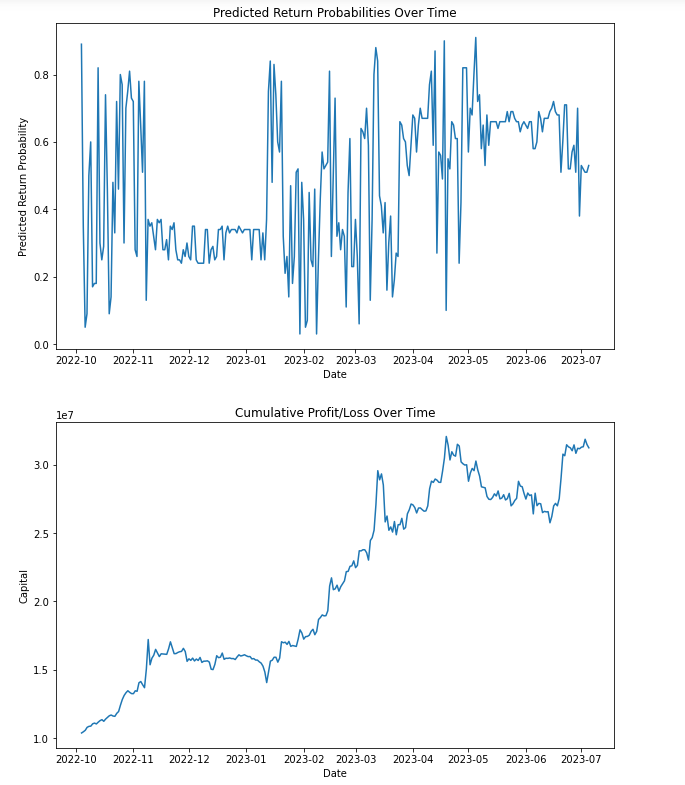
\includegraphics[scale=0.65]{fig22.jpg}
\end{figure}

\begin{figure}[H]
\centering
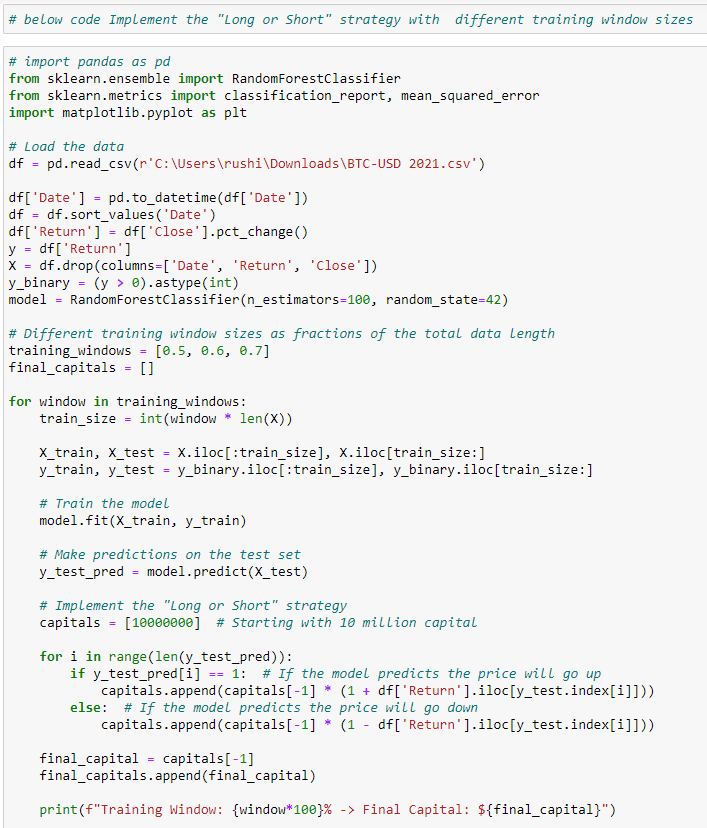
\includegraphics[scale=0.65]{fig23.jpg}
\end{figure}

\begin{figure}[H]
\centering
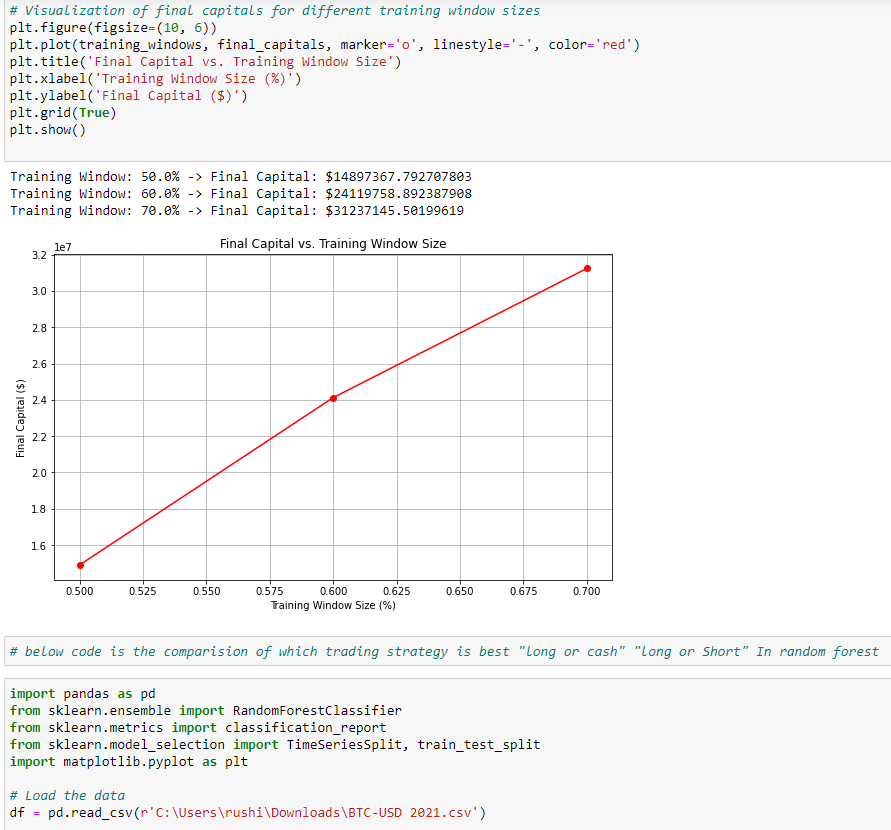
\includegraphics[scale=0.65]{fig24.jpg}
\end{figure}

\begin{figure}[H]
\centering
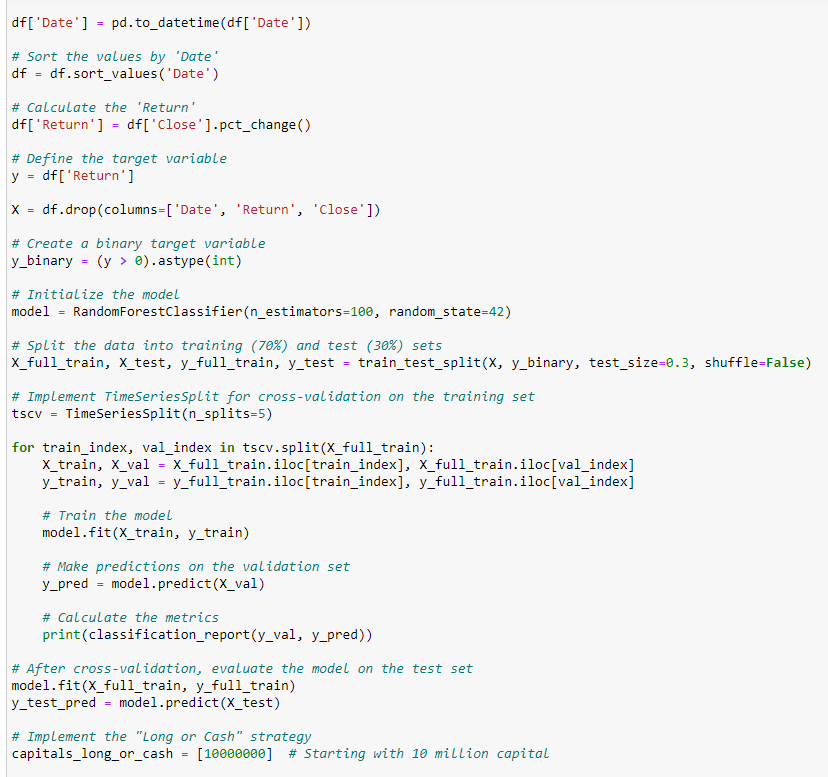
\includegraphics[scale=0.65]{fig25.jpg}
\end{figure}
\begin{figure}[H]
\centering
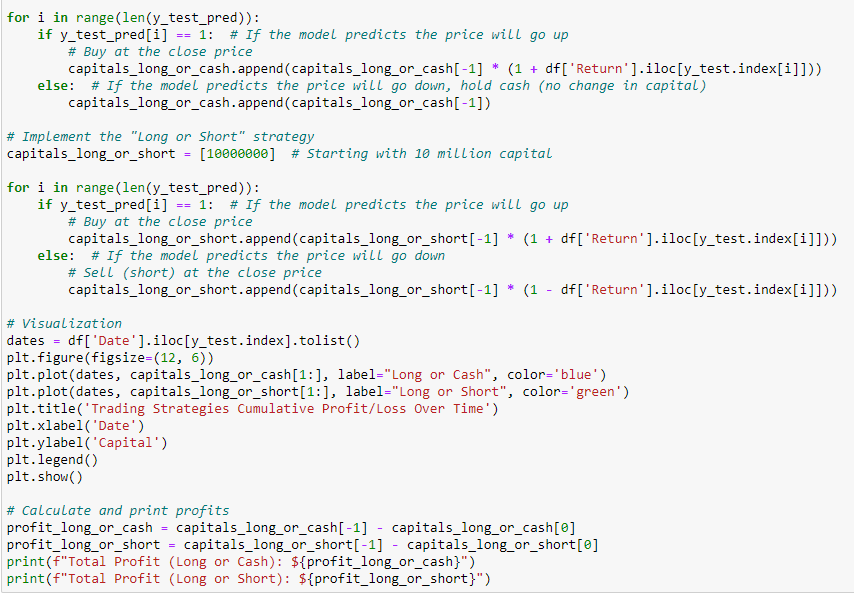
\includegraphics[scale=0.65]{fig26.jpg}
\end{figure}

\begin{figure}[H]
\centering
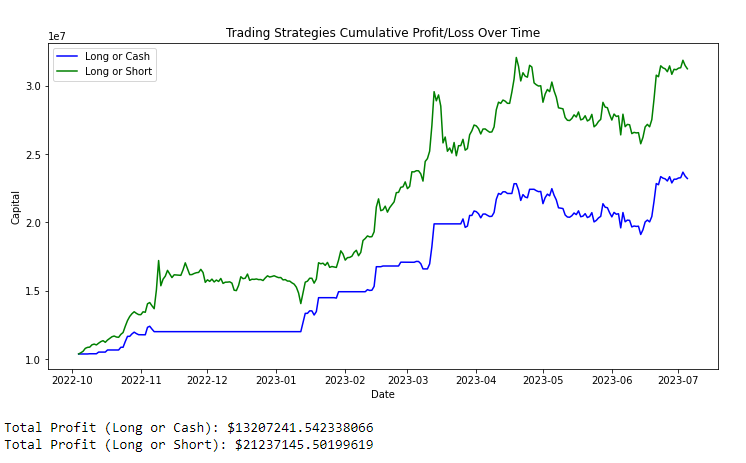
\includegraphics[scale=0.65]{fig27.jpg}
\end{figure}

\begin{figure}[H]
\centering
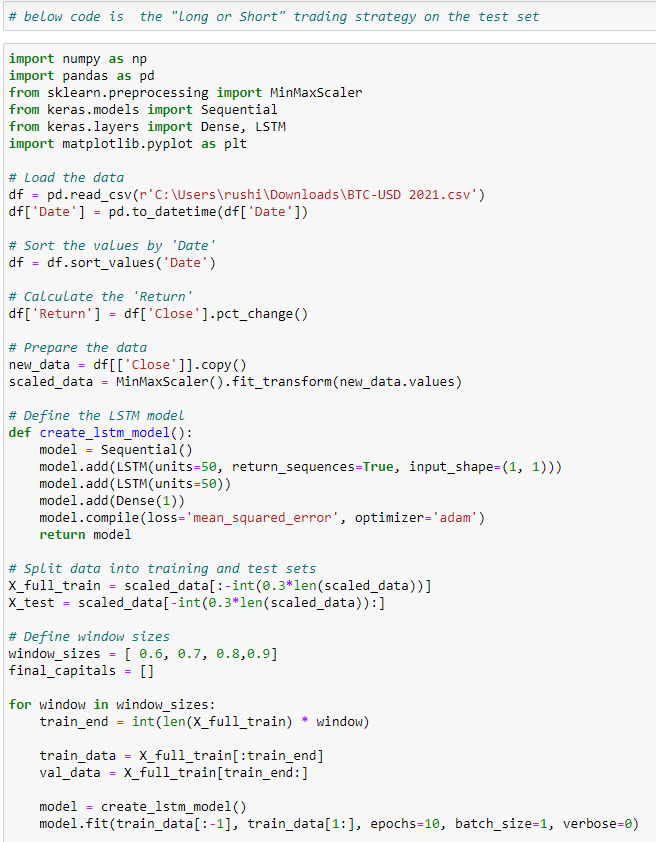
\includegraphics[scale=0.65]{fig28.jpg}
\end{figure}

\begin{figure}[H]
\centering
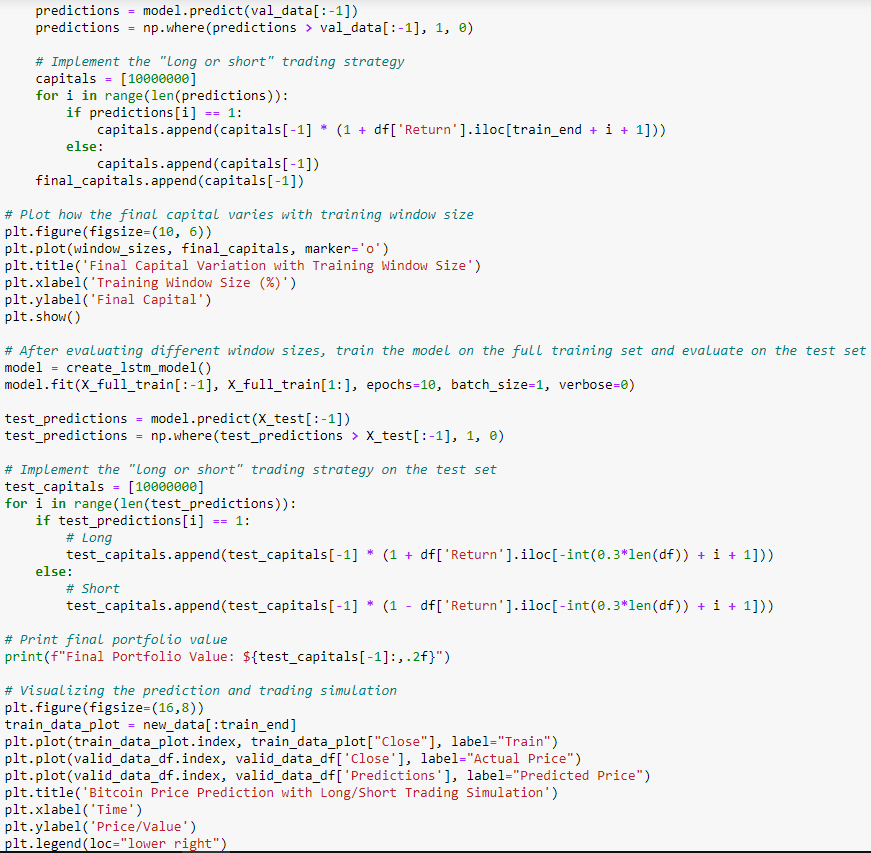
\includegraphics[scale=0.65]{fig29.jpg}
\end{figure}

\begin{figure}[H]
\centering
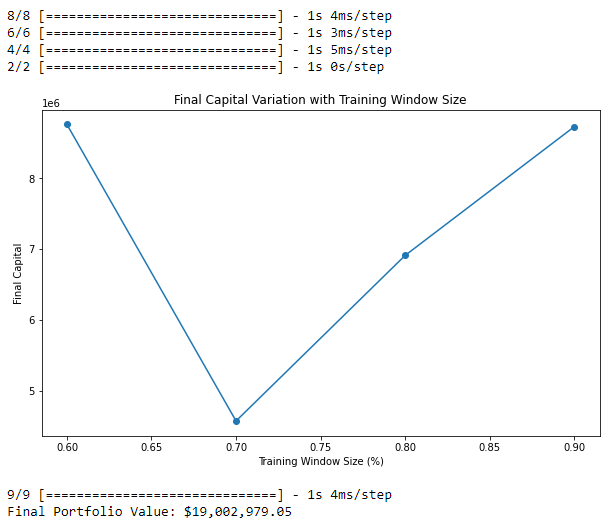
\includegraphics[scale=0.65]{fig30.jpg}
\end{figure}

\begin{figure}[H]
\centering
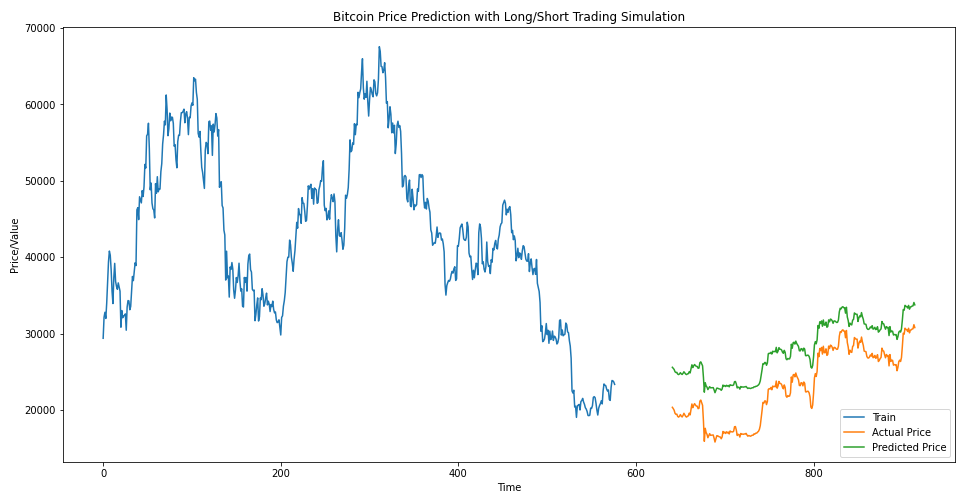
\includegraphics[scale=0.65]{fig31.jpg}
\end{figure}

\begin{figure}[H]
\centering
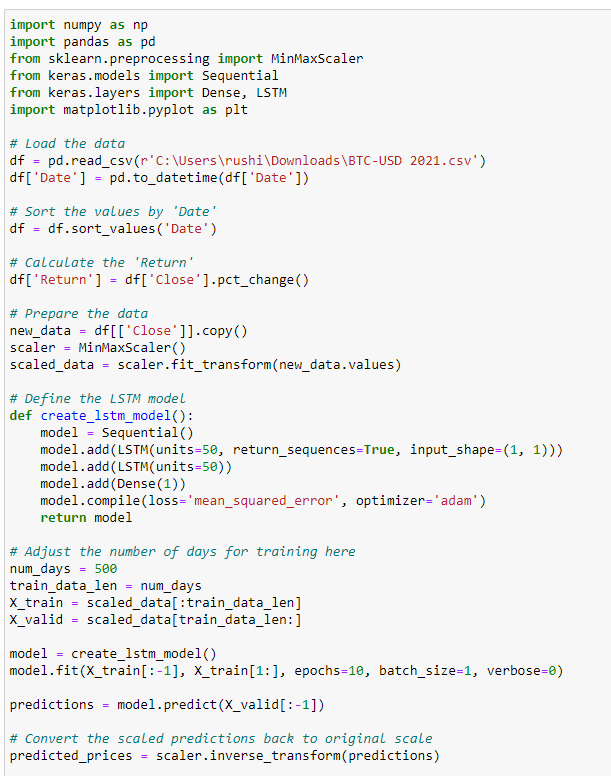
\includegraphics[scale=0.65]{fig32.jpg}
\end{figure}

\begin{figure}[H]
\centering
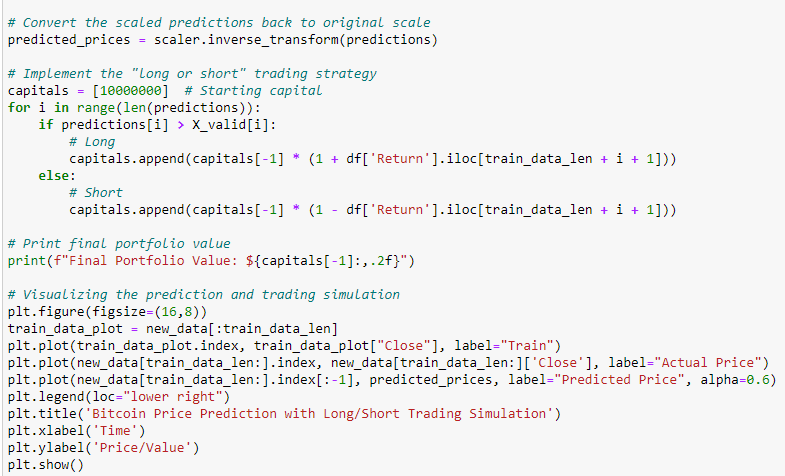
\includegraphics[scale=0.65]{fig33.jpg}
\end{figure}

\begin{figure}[H]
\centering
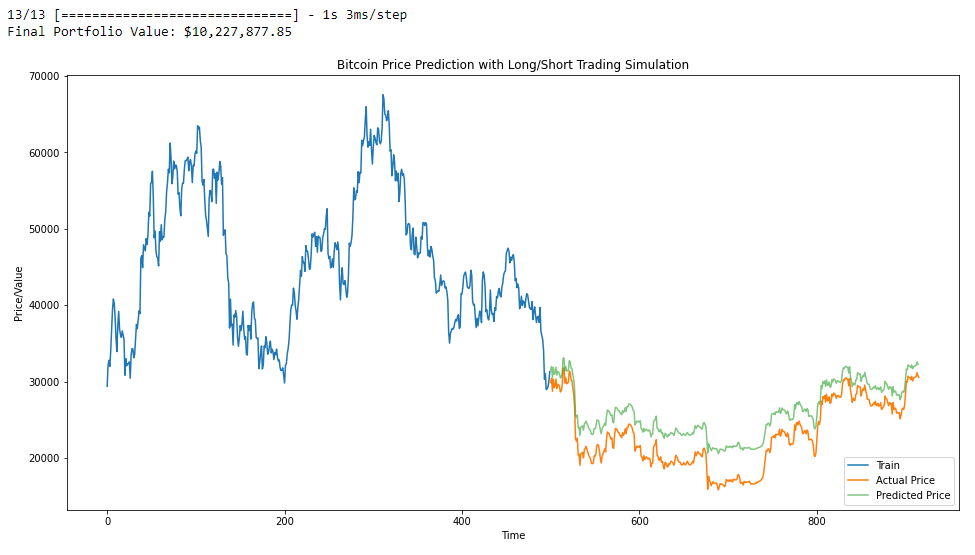
\includegraphics[scale=0.65]{fig34.jpg}
\end{figure}